\documentclass[border=8pt]{standalone}
\usepackage{tikz}
\usetikzlibrary{arrows.meta,positioning,calc,fit}
\begin{document}
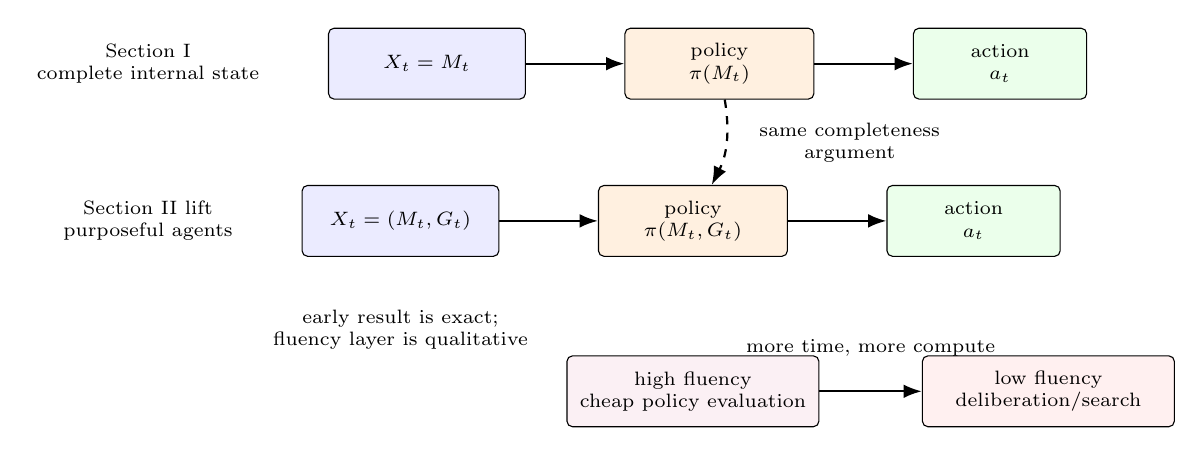
\begin{tikzpicture}[
  box/.style={draw, rounded corners=2pt, align=center, minimum width=2.55cm, minimum height=0.9cm, font=\scriptsize},
  state/.style={draw, rounded corners=2pt, align=center, minimum width=2.5cm, minimum height=0.9cm, font=\scriptsize, fill=blue!8},
  policy/.style={draw, rounded corners=2pt, align=center, minimum width=2.4cm, minimum height=0.9cm, font=\scriptsize, fill=orange!12},
  action/.style={draw, rounded corners=2pt, align=center, minimum width=2.2cm, minimum height=0.9cm, font=\scriptsize, fill=green!8},
  note/.style={align=center, font=\scriptsize},
  arr/.style={-Latex, thick},
  dasharr/.style={-Latex, thick, dashed}
]

\node[note] (sec1label) {Section I\\complete internal state};
\node[state, right=0.75cm of sec1label] (m) {$X_t=M_t$};
\node[policy, right=1.25cm of m] (pi1) {policy\\$\pi(M_t)$};
\node[action, right=1.25cm of pi1] (a1) {action\\$a_t$};
\draw[arr] (m) -- (pi1);
\draw[arr] (pi1) -- (a1);

\node[note, below=1.25cm of sec1label] (sec2label) {Section II lift\\purposeful agents};
\node[state, right=0.75cm of sec2label] (x) {$X_t=(M_t,G_t)$};
\node[policy, right=1.25cm of x] (pi2) {policy\\$\pi(M_t,G_t)$};
\node[action, right=1.25cm of pi2] (a2) {action\\$a_t$};
\draw[arr] (x) -- (pi2);
\draw[arr] (pi2) -- (a2);

\node[box, fill=purple!6, below=1.25cm of pi2, minimum width=3.2cm] (implicit) {high fluency\\cheap policy evaluation};
\node[box, fill=red!6, right=1.3cm of implicit, minimum width=3.2cm] (explicit) {low fluency\\deliberation/search};
\draw[arr] (implicit) -- (explicit);
\node[note, above=0.32cm of $(implicit)!0.5!(explicit)$] {more time, more compute};

\draw[dasharr] (pi1) to[bend left=18] (pi2);
\node[note, right=0.55cm of $(pi1)!0.5!(pi2)$] {same completeness\\argument};
\node[note, below=0.55cm of x] {early result is exact;\\fluency layer is qualitative};

\end{tikzpicture}
\end{document}
